% 固定来源 PDF 印刷页 77 第 23 题双曲线、渐近线及圆的矢量示意。
% 曲线和圆为结构示意，比例与切点位置不作为题设数据。
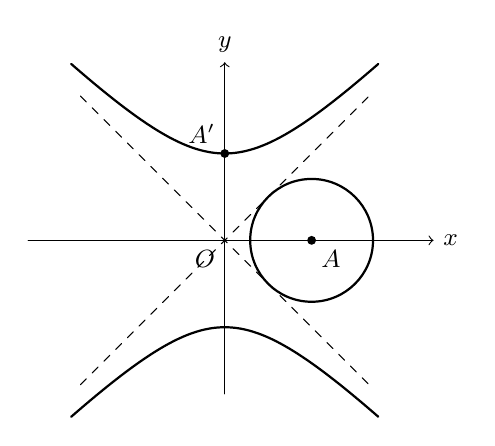
\begin{tikzpicture}[x=.78cm,y=.78cm,font=\small,line cap=round,line join=round]
  \draw[->] (-3.2,0)--(3.4,0) node[right] {$x$};
  \draw[->] (0,-2.5)--(0,2.9) node[above] {$y$};
  \draw[dashed] (-2.35,-2.35)--(2.35,2.35);
  \draw[dashed] (-2.35,2.35)--(2.35,-2.35);
  \draw[thick,domain=-2.5:2.5,samples=70,variable=\x]
    plot (\x,{sqrt(\x*\x+2)});
  \draw[thick,domain=-2.5:2.5,samples=70,variable=\x]
    plot (\x,{-sqrt(\x*\x+2)});
  \draw[thick] (1.414,0) circle (1);
  \fill (1.414,0) circle (1.6pt); \node[below right] at (1.414,0) {$A$};
  \fill (0,1.414) circle (1.6pt); \node[above left] at (0,1.414) {$A'$};
  \node[below left] at (0,0) {$O$};
\end{tikzpicture}
